% latex article template

% cheat sheet(eng): http://www.pvv.ntnu.no/~walle/latex/dokumentasjon/latexsheet.pdf
% cheat sheet2(eng): http://www.pvv.ntnu.no/~walle/latex/dokumentasjon/LaTeX-cheat-sheet.pdf
% reference manual(eng): http://ctan.uib.no/info/latex2e-help-texinfo/latex2e.html

% The document class defines the type of document. Presentation, article, letter, etc. 
\documentclass[12pt, a4paper]{article}

% packages to be used. needed to use images and such things. 
\usepackage[pdfborder=0 0 0]{hyperref}
\usepackage[utf8]{inputenc}
\usepackage[english]{babel}
\usepackage{graphicx}
\PassOptionsToPackage{hyphens}{url}

% hides the section numbering. 
\setcounter{secnumdepth}{-1}

% Graphics/image lications and extensions. 
\DeclareGraphicsExtensions{.pdf, .png, .jpg, .jpeg}
\graphicspath{{./images/}}

% Title or header for the document. 
\title{
	TIØ4116, Exercise 10. 
}
% Author
\author{
	Magnus L. Kirø \\
}
\date{\today}

\begin{document}
\maketitle
\pagenumbering{arabic}

\section{Task 1}
\paragraph{A}
We want a price p that is less than a, so we assume that p=2/3a resulting in
q=1/3a. Giving the us a linear income graph of in=N*(1/3a). 

see fig1. 

% image example. 
\begin{figure}[htb]
    \centering
    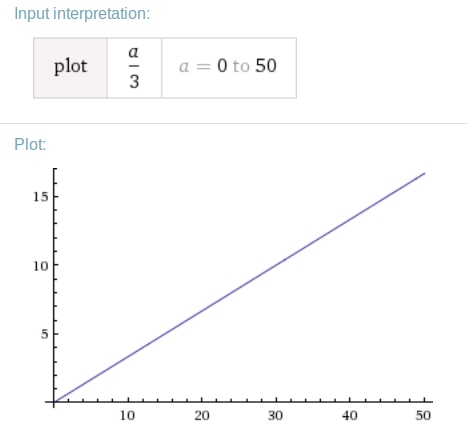
\includegraphics[width=\textwidth]{plot} 
    \label{fig:plot}
    \caption{}
Fig1: The graph shows the linear income graph, where y is the number of visitors and a
is the constant of the quantity function. 
\end{figure}

\paragraph{B}
With the second pricing policy I would choose A an p so that a>(p+A). Assuming
A=1/3a, and p=1/3a we get a positive q, which means we will have visitors in
the amusement park. With A=p=1/3a we get the same income graph as in task 1a,
resulting in Fig1.  

\paragraph{C}
I would choose price policy 2. Because the price for the visitors are
distributed, making it possible to distribute maintenance of rides over p, and
park maintenance over A. As both policies depend on a we can get the same
profit from both models.

\paragraph{D}
Deadweight loss occurs when the price is higher than the price ceiling. In our
case the price ceiling is a. If p is greater than a we will have negative q,
resulting in no customers and no income. The value of the deadweight is the
amount of visitors that won't come when the price is increased from the price
ceiling. 

\section{Task 2}
\paragraph{A}
The CEO would choose project 2. This project gives the highest accumulated
utility by probability. The shareholders would want the same project, as this
gives the highest probable return given the CEO they have chosen. The value of
alpha would not change this. But it might change the choice of reward for the
CEO. 

\paragraph{B}
Another CEO with another utility function might choose differently. This
depends on the utility function. Given a utility function with a second
variable depending on the probability, we would get very different  results. 

\paragraph{C}
Given the options reward model, and the fact that the CEO only gets reward of 1
when A is less than 30, the CEO would choose project 1. Project 1 gives the
highest probability per utility of achieving the higher value of A. Therefore
maximizing the reward. The value of beta does not affect the decision, only the
final numerical value of the reward. It will still be maximized. 

\section{Task 3}
\paragraph{A}
The duration of a consol is unlimited. The interest is set at time=0. The
duration of a treasury is 1, it is set every yea, it is set every year.

\paragraph{B}
To even out the investments, 455000 should be invested in consols, and 454000
should be invested in treasuries. This results in 1000000 after two years. 

\paragraph{C}
By increasing the interest by 2\% after two years we see that we could have
invested less in both  options. Reducing the investments to 435000 in each we
still get more than 100000 pounds.

Reducing the \% interest we should have invested more in consols, and less in
treasuries to achieve the same result. 

\section{Task 4}
\paragraph{A}
The risk-neutral player should pay 8. That is when the probability of winning
becomes so small that it's not worth it any more.

\paragraph{B}
The expected value of this lottery is very little. It is unlikely to win after
five tosses. The difference from five tosses to a price of 8 is 24.  

\paragraph{C}
For a risk averse person the certainty equivalent would be 2. It is the lowest
amount of reward that would make the person take the risk. 

\paragraph{D}
Nothing. In the long run it's better to keep any amount of money than bet it on
odds that doesn't insure payback. 

\paragraph{E}
Same as task 4d.

\end{document}
This is never printed
